%Num-Projekt1, Amanda ? , Christoph Mayer

\documentclass[a4paper,11pt,bibliography=totoc,listof=totoc,headinclude=true,cleardoublepage=empty,oneside]{scrbook}
% Option "oneside" für einseitigen Druck. Weglassen, falls die Arbeit doppelseitig gedruckt wird
\usepackage{graphicx} 
\usepackage[english,ngerman]{babel}
\usepackage[utf8]{inputenc}
%\usepackage{fullpage}
\usepackage{ifthen}
\usepackage{color}
\usepackage{amsmath,amsthm,amssymb,amsfonts}
\usepackage{graphicx}
\usepackage{amsmath}
\usepackage{mathtools}
\usepackage{tikz}
% links in pdf
\usepackage[unicode,colorlinks=true,pagebackref=false]{hyperref}
\usepackage{listings}
%\usepackage{maplestd2e}
% Zum Druck verwende schwarze Links!
%\usepackage[unicode,colorlinks=true,linkcolor=black,citecolor=black,urlcolor=black,pagebackref=false]{hyperref} 
% colorlinks=false umrahmt Links statt einzufaerben, 




% document style
\KOMAoptions{footinclude=false} % Fusszeile wird nicht zu Satzspiegel gezaehlt
\KOMAoptions{headsepline=true} % Trennlinie zwischen Kopfzeile und Text
\KOMAoptions{DIV=12} % beeinflusst Satzspiegel
\KOMAoptions{BCOR=8mm} % Bindekorrektur
\pagestyle{headings} % mit Kopfzeilen

\recalctypearea % berechne Satzspiegel neu

\definecolor{change}{rgb}{0,.55,.55}
\definecolor{change2}{rgb}{0,0,0}
\definecolor{change3}{rgb}{0.5,0,0}

\def\revision#1{{\color{red}#1}}

\lstset{ 
	language=Matlab, 
	showstringspaces=false}

\newcommand{\code}[1]{\texttt{\color{change}#1}}


%%%%%%%%%%%%%%%%%%%%%%%%%%%%%%%%%%%%%%%%%%%%%%%%%%%%%%%%%%%%%%%%%%%%%%%%%%%%%%%%%%%%%%%%%%%%%%%%%%%%%%%%%%%%%%
%%%%%%%%%%%%%%%%%%%%%%%%%%%%%%%%%%%%%%%%%%%%%%%%%%%%%%%%%%%%%%%%%%%%%%%%%%%%%%%%%%%%%%%%%%%%%%%%%%%%%%%%%%%%%%
%%%%%%%%%%%%%%%%%%%%%%%%%%%%%%%%%%%%%%%%%%%%%%%%%%%%%%%%%%%%%%%%%%%%%%%%%%%%%%%%%%%%%%%%%%%%%%%%%%%%%%%%%%%%%%
%%%%%%%%%%%%%%%%%%%%%%%%%%%%%%%%%%%%%%%%%%%%%%%%%%%%%%%%%%%%%%%%%%%%%%%%%%%%%%%%%%%%%%%%%%%%%%%%%%%%%%%%%%%%%%

\begin{document}


\pagenumbering{arabic}
\selectlanguage{ngerman}

\begin{titlepage}
	%\vspace*{-2cm}
	\begin{center}
	%	\includegraphics[width=0.45\textwidth]{TULogo.eps}
		\vskip 1cm%
		{\LARGE N~\Large U~M~E~R~I~K}
		\vskip 8mm
		{\huge\bfseries Projekt 1}
		\vskip 1cm
		
		{\Large\bfseries Name des Tutors: Johann Faschingleitner}\\[1ex]
		\vskip 0.5cm
		{\Large\bfseries Name der Autoren:}\\[1ex]
		\vskip 0.5cm
		Christoph Mayer
		\vskip 0.5cm
		Matrikelnummer: e01425430\\[1ex]
		\vskip 0.5cm
		Amanda Schöfl
		\vskip 0.5cm
		Matrikelnummer: e0271473\\[1ex]
	\end{center}
\end{titlepage}

\cleardoublepage
	
\chapter*{Aufgabe 3} %\chapter*{Acknowledgement}
\thispagestyle{empty}
\selectlanguage{ngerman} %\selectlanguage{english}

\subsubsection{3.1 Aufgabenstellung}
Basierend auf einer 1D Quadratur kann durch Bildung des Tensorproduktes eine 2D Quadratur erzeugt werden. Sei dazu $f:	\mathbb{R} ^2 \to \mathbb{R}$ eine auf dem Einheitsqudrat $Q:=[0,1]\times[0,1]$ integrierbare Funktion, dann gilt (mittels Fubini)
		
\begin{equation}\label{equ:integral}
\begin{array}{rccll}
	\int\limits_{\hat{Q}}f(x,y)d(x,y)&=&\int_0^{1}\Big(\int_0^{1}f(x,y)dx\Big)dy&=&\\
	&=&\int_0^{1}\Big(\sum_{i=0}^n\alpha_i f(x_i,y)\Big)dy &=&\\ 
	&=&\sum_{i=0}^n \alpha_i \int_0^{1} f(x_i,y)dy&=&\\
	&=&\sum_{i=0}^{n} \alpha_i\Big(\sum_{j=0}^{n} \alpha_j f(x_i,y_i)\Big)&=&\sum_{i,j=0}^{n} \alpha_i\alpha_j f(x_i,y_j),\\
\end{array}
\end{equation}
wobei $\{\alpha_i: i=0,...n\}$ und  $\{x_i,y_j : i,j=0,...n\}$ die 1D Quadraturgewichte und -knoten sind. Somit kann man mit den bereits bekannte 1D Quadraturen auch Integrale am Einheitsquadrat numerisch berechnen. Implementieren Sie mit Hilfe des zur Verfügung gestellten Programms \textbf{gauss(n)} eine Funktion \textbf{quadInt(f,n)} die $\int_{\hat{Q}}f(x,y)d(x,y) $ berechnet. Für welche n wird ein Polynom $ p \in \prod_{2}^k:=span\{x^iy^j:0 \leq i,j\leq k \} $ exakt integriert?

\subsubsection{3.1 Durchführung}

Die folgende Implementierung der Funktion \textbf{quadInt}, hat die Inputparameter
\begin{itemize}
	\item \code{f} ein Function Handle einer Funktion mit oben beschriebenen Eigenschaften,
	\item \code{n} der Grad der Gaußquadratur.
\end{itemize} 
Sie gibt den approximierten Wert des Integrals der übergebenen Funktion auf $\hat{Q}$ zurück.
{
	\color{change}		
%\lstset{ 
%	language=Matlab, 
%	showstringspaces=false}
\lstinputlisting{quadInt.m} 
		
%		\begin{lstlisting}
%
%		\end{lstlisting}
% Was tut das??
}
Widmen wir uns jetzt noch der Frage für welche $n$ ein Polynom $ p \in \prod_{2}^k:=span\{x^iy^j:0 \leq i,j\leq k \} $ exakt integriert wird.		
Wir wissen dass für 1D Quadraturen Polynome vom Grad $2n+1$ exakt numerisch berechnet werden können. Da in (0.1) lediglich die Gauß-Quadratur 2-mal hintereinander eindimensional durchgeführt wird, gilt, dass i=2n+1 und j=2n+1 die höchsten Grade sind, für welche die 2D Quadratur exakt numerisch berechnet werden kann.


\subsubsection{3.2 Aufgabenstellung}
		Da zum Beispiel bei der Finite-Element-Methode eine Quadratur auf Dreiecken benötigt wird, verwendet man gerne die \textit{Duffy-Transformation} um die Quadratur auf dem Einheitsquadrat \^{Q} auf das Referenzdreieck \^{T} mit den Eckpunkten $ (0,0),(1,0)$ und $ (0,1)$ zu transformieren.
		Die \textit{Duffy-Transformation} ist definiert als:
		
		\begin{equation} 
		\Psi = \begin{cases} 
		\hat{Q} \to \hat{T} \\
		(s,t) \mapsto (s,(1-s)t)
		\end{cases} 
		\end{equation} 
		\\
		Implementieren Sie mithilfe der \textit{Duffy-Transformation} die Funktion \textbf{trigInt(f,n)}, sodass Sie Integrale auf \^{T} berechnen können.
		\textit{Hinweis}: Verwenden Sie dazu die Substitutionsregel Satz 7.34 (Transformationssatz für Integrale) aus dem Analysis-Skript von Professor Engl.
		
	
	\vspace{0.5cm}
	
	\subsubsection{3.2 Durchführung}
\setlength{\fboxsep}{1em}
\fbox{
	\parbox{35.5em}{Transformationssatz für Integrale:
		
		Es sei $\Omega \in \mathbb{R}$ eine offene Menge und $\Phi:\Omega \to \Phi(\Omega) \in \mathbb{R}^d$ ein Diffeomorphismus. Dann ist die Funktion $f$ auf $\Phi(\Omega)$ genau dann integrierbar, wenn die Funktion $x \mapsto f(\Phi(x)) |det(D\Phi(x))| $ auf $\Omega$ integrierbar ist.
		In diesem Fall gilt: \linebreak
	\begin{equation}
		\int_{\Phi(\Omega)}f(y)dy = \int_{\Omega}f(\Phi(x))|det(D\Phi(x))|dx.
	\end{equation}
	
		Dabei ist $D\Phi(x)$ die Jacobi-Matrix und $det(D\Phi(x))$ die Funktionaldeterminante  von $\Phi$,also $Df(\Phi)=\Big(\frac{\partial f_i}{\partial x_j}(x)\Big)_{i,j=1,...,n}$}}
\vspace{0.5cm}
		% Funktionaldeterminante anpassen
		
		
Auf unseren Fall angewandt mit $\Omega=\hat{Q}$, $\Psi=\hat{T}$, sowie mit der Funktionaldeterminante 
		
\begin{equation*}
	det \hat{T} = |det		
	\left(
	\begin{array}{cc}
	1 & -t \\
	0 & (1-s)\\
	\end{array}
	\right)| = |(1-s)| 
\end{equation*}

ergibt sich
		\vspace{10mm}
	

	

			
			\begin{equation} \label{eq1}
			\begin{split}
	\int_{\hat{T}}f(x,y)d(x,y) &= \int_{\hat{Q}}f(s,(1-s)t)|(1-s)|d(t,s) \\
		&= \sum_{{i,j=0}}^{n}\alpha_i \alpha_j f(s_i,(1-s_i)t_j)|(1-s_i)| 
			\end{split}
			\end{equation}
	
		
		\vspace{3mm}
		Dadurch ergibt sich insgesamt: 
		\\
		\vspace{-2mm}
	
		\begin{equation}
		trigInt(f,n) = quadInt(f\circ(s,t) \mapsto (s,(1-s)t))*(1-s)
		\end{equation}
		
		
		

		\vspace{4mm}		
	
		
		
		\color{change2}
		\subsubsection{3.2 Code}
		Die folgende Implementierung der Funktion \textbf{trigInt}, hat die Inputparameter
		\begin{itemize}
			\item \code{f} ein Function Handle einer Funktion mit oben beschriebenen Eigenschaften,
			\item \code{n} der Grad der Gaußquadratur.
		\end{itemize} 
		Sie gibt den approximierten Wert des Integrals nach der Transformation auf  $\hat{T}$ auf das Referenzdreieck mit den Eckpunkten $(0,0),(0,1),(1,0)$ zurück.
		
\color{change}
		\lstset{ 
			language=Matlab, 
			showstringspaces=false}
		
		\lstinputlisting{trigInt.m} 
		\begin{lstlisting} 
		
		
		\end{lstlisting}
		
	\color{change2}
		
		
		\subsubsection{3.3 Aufgabenstellung}
		\vspace{1mm}
		
		
		 Erweitern Sie unter Verwendung einer affinen Transformation $\Phi_T:\hat{T} \to T$ Ihre Implementierung von $\textbf{duffyInt}$, um auch Integralen auf beliebigen Dreiecken T berechnen zu können. 
		Für welche n wird ein Polynom $ p \in \prod_{2}^k:=span\{x^iy^j:0 \leq i+j\leq k \} $ exakt integriert? \\
		
		\vspace{-3mm}
		\textit{Hinweis:} Sie können die Implementation Ihrer Transformation testen, indem Sie das Integral über $f \equiv1$ numerisch berechnen und mit der analytisch bestimmten Fläche des Dreiecks T vergleichen.
		
		\vspace{5mm}
		\subsubsection{3.3 Durchführung}
		
		Anstatt einer affinen Transformation von $ \Phi_{\hat{T}}:\hat{T} \to T$ verwenden wir eine affine Transformation $\Phi:\hat{Q} \mapsto T$. \\
		
		Wir nehmen nun ein beliebiges Dreieck T mit \\
		
		 $a=\left(
		\begin{array}{ccc}
		a_1 \\
		a_2\\
		\end{array}
		\right)$, $b=\left(
		\begin{array}{ccc}
			b_1 \\
			b_2\\
		\end{array}
		\right)$, $c=\left(
		\begin{array}{ccc}
			c_1 \\
			c_2\\
		\end{array}
		\right)$, 
		\vspace{3mm}
		
		
		
		v=$\left(
		\begin{array}{ccc}
		(1-s)*a_1+ s*c_1\\
		(1-s)*a_2+s*c_2\\
		\end{array}
		\right)$ 	und w=$\left(
		\begin{array}{ccc}
			(1-s)*b_1+ s*c_1\\
			(1-s)*b_2+s*c_2\\
		\end{array}
		\right)$
		
		\vspace{5mm}
		zur Hand, wobei die Vektoren $\vec{v}$ und $\vec{w}$ Konvex-Kombinationen der Punkte $a$ und $b$ sind:
		
		\vspace{4mm}
		
	\hspace{3.6cm}	\begin{tikzpicture}
		%Koordinaten für die Beschriftung 
		\coordinate[label=left:$a$]  (A) at (5,0); 
		\coordinate[label=right:$b$] (B) at (10,2); 
		\coordinate[label=above:$c$] (C) at (6,2.5); 
		
		\draw[->] (A) -- (B) -- (C) -- (A);
		%warum funktioniert vektor nicht?
		\path [->] 
		(A) edge node [left]{$\vec{v}$} (C)   ;
		\path[->]
		(B) edge node [above]{$\vec{w}$} (C) ;  
		
		\end{tikzpicture}
	
	\vspace{3mm}
		Das Dreieck kann nun wie folgt dargestellt werden:
		
		\vspace*{2mm}
		\begin{equation*}
			(1-t)v+s*w)
		\end{equation*}	
			
		und die angepasste \textit{Duffy-Transformation} lautet wie folgt: \\
		
	
		
		\vspace*{1mm}
		
		\begin{equation*}
				(s,t) \mapsto \left(
				\begin{array}{ccc}
				a_1 + s*(c_1-a_1)+ t*(b_1-a_1) + st(a_1-b_1)\\
				a_2 + s(c_2-a_2) + t(b_2-a_2) + st(a_2-b_2)\\
				\end{array}
				\right).
		\end{equation*} \\
		 \vspace*{5mm}
		Durch Proberechnung anhand des Beispiel unseres Referenzdreiecks, mit \\  \hspace*{0mm} $a=\left(
		\begin{array}{ccc}
		0 \\
		0\\
		\end{array}
		\right)$, $a=\left(
		\begin{array}{ccc}
		0 \\
		1\\
		\end{array}
		\right)$, $c=\left(
		\begin{array}{ccc}
		1\\
		0\\
		\end{array}
		\right)$ folgt:
		
		\vspace{3mm}
		\hspace{4.3cm}

		\vspace{2mm}
		
		
		$(s,t) \mapsto  c=\left(
		\begin{array}{ccc}
			t-st\\
			s\\
		\end{array}
		\right) = \left(
		\begin{array}{ccc}
			t*(1-s)\\
			s\\
		\end{array}
		\right)$. \newline
		
		Damit ist unsere Transformation korrekt und wir können mit der Implementierung des Codes voranschreiten:
	
	\vspace{3mm} 
		
		
			\subsubsection{3.3 Code}
			Die folgende Implementierung der Funktion \textbf{duffyInt}, hat die Inputparameter
			\begin{itemize}
				\item \code{f} ein Function Handle einer Funktion mit oben beschriebenen Eigenschaften,
				\item \code{n} der Grad der Gaußquadratur.
				\item \code{$a_1,a_2$} : Koordinaten des Punktes a
				\item \code{$b_1,b_2$} : Koordinaten des Punktes b
				\item \code{$c_1,c_2$} : Koordinaten des Punktes c
			\end{itemize} 
			Sie gibt den approximierten Wert des Integrals nach der Transformation auf ein beliebiges Dreieck mit den Eckpunkten (a,b,c) zurück: \\
		
		\color{change}
		\lstset{ 
			language=Matlab, 
			showstringspaces=false}
		
		
		
		\lstinputlisting{duffyInt.m} 
		\begin{lstlisting} 
		
		
		\end{lstlisting}
		
		\begin{flushleft}
		
		\color{change2}
		\textbf{Widmen wir uns nun noch der Frage wann ein Polynom $ p \in \prod_{2}^k:=span\{x^iy^j:0 \leq i+j\leq k \} $ exakt integriert werden kann:}
		
		Da wir nur die Hülle $span\{x^iy^j:0 \leq i+j \leq k\}$ betrachten, können wir das Polynom $p=x^iy^j$ mit den höchstmöglichen Graden $i$ und $j$ heranziehen.
		
		Sei nun $ p \in \prod_{2}^k \Rightarrow \int_{\hat{T}}^{} p(x,y)d(x,y) = 
		\int_{\hat{Q}}^{} p(\Phi(x),\Phi(y)) * det|d\Phi| d(s,t)$ .
		
		Für $p=x^iy^j$ lautet die Transformation wie folgt:
		
		$p(\Phi(x),\Phi(y)) = (\alpha_1+s\alpha_2+t\alpha_3+st\alpha_4)^i(\beta_1+s\beta_2+t\beta_3+st\beta_4)^j$. \\
		
		Aus diesem Ausdruck lesen wir heraus dass der höchste Term $\delta_0s^it^is^jt^j = s^{(i+j)}t^{(i+j)}\delta_0$	mit einer Konstanten $\delta_0$ ist, die in diesem Fall vernachlässigt werden kann.
			
			Hingegen ist der höchste Term der Funktionaldeterminante $det|D\Phi|$ $\delta_1st$.
			
			
			Somit ist der größte Term von
			 $\int_{\hat{Q}}^{} p(\Phi(x),\Phi(y)) * det|d\Phi| d(s,t)$ 
			 vom Grad
			 $\delta^{i+j+1}t^{i+j+1}$.
			 Da $i+j+1\leq2n+1$ gefordert wird,  $i+j\leq2n$.
			 			
			
		\end{flushleft}
\vspace{1cm}
		\color{black}
		\subsubsection{3.4 Aufgabenstellung} 
		 Erweitern Sie Ihre Implementierung von \textbf{quadInt(f,n)} zur Berechnung von Integralen auf beliebigen konvexen Vierecken $ Q=conv{(a1,a2),(b1,b2),(c1,c2),(d1,d2)} $. Verwenden Sie dazu eine eine Transformation der Form:
		
			\begin{equation} 
			\Psi_{\hat{Q}} = \begin{cases} 
			\hat{Q} \to Q \\
			(u,v) \mapsto
			
		 \left(
		  \begin{array}{ccc}
		  \alpha_1 + \alpha_{2}u + \alpha_{3}v +\alpha_{4}uv \\
		  \beta_1+\beta_{2}u+beta_{3}v+\beta_{4}uv \\
		  \end{array}
		  \right)

			\end{cases} 
			\end{equation} \\
			
			\color{change2}
\begin{flushleft}		mit den Konstanten $\alpha_i$,$\beta_i \in \mathbb{R}$. Überlegen Sie sich, warum nicht-konvexe Vierecke unzulässig sind.\end{flushleft} 
		\vspace*{3mm}
		
		\subsubsection{3.4 Durchführung}
		
		Wir sollen nun nun unsere Implementierung auf beliebige konvexe Vierecke \linebreak
		
		\hspace*{3.5cm}\begin{tikzpicture} 
		%Koordinaten für die Beschriftung 
		\coordinate[label=left:$a$]  (A) at (0,0); 
		\coordinate[label=left:$b$] (B) at (2,3); 
		\coordinate[label=above:$c$] (C) at (3.5,3.5);
		\coordinate[label=right:$d$] (D) at (3.5,1); 
		
		\draw (A) -- (B) -- (C) -- (D) -- (A);
		\path [->] 
		(A) edge node [below]{$\vec{v}$} (D)   
		(B) edge node [above]{$\vec{w}$} (C)   
		; 
		\end{tikzpicture}
		
		erweitern.
		
		
		Die Konvexkombination funktioniert analog zu der in Aufgabe $(3.3)$: \\ \\
		
		\hspace{4cm}$\vec{v}*(1-t)+\vec{w}*t$
		\color{change2}
		mit\\ \\
		
	\hspace{2.6cm}	$\vec{v} = a*t+d*(1-t)$ \color{change2}und
		$\vec{w} = b*t+c*(1-t)$ . \\
		\color{change2}
		\hspace{2mm}
		\\Wenn man dies ausmultipliziert ergibt das genau die Transformation die in der Aufgabenstellung angegeben ist. \\
		\begin{flushleft}
	
		Letztlich widmen wir uns der Frage wir nur konvexe Vierecke verwenden dürfen:\\
		Da die Vektoren konvexkombiniert werden ist es augenscheinlich dass nur konvexe Vierecke für unsere Transformation geeignet sind..
		
			\end{flushleft}
		\subsubsection{3.4 Code}
			Die folgende Implementierung der Funktion \textbf{quadInt2}, hat die Inputparameter
			\begin{itemize}
				\item \code{f} ein Function Handle einer Funktion mit oben beschriebenen Eigenschaften,
				\item \code{n} der Grad der Gaußquadratur.
				\item \code{$a_1,a_2$} : Koordinaten des Punktes a
				\item \code{$b_1,b_2$} : Koordinaten des Punktes b
				\item \code{$c_1,c_2$} : Koordinaten des Punktes c
				\item \code{$d_1,d_2$} : Koordinaten des Punktes d
			\end{itemize} 
		\color{change}
		\lstset{ 
			language=Matlab, 
			showstringspaces=false}
		
		\lstinputlisting{quadInt2.m} 
		\begin{lstlisting} 
		
		
		\end{lstlisting}
		
		
		
		
		
		\color{change2}
		\subsubsection{3.5 Aufgabenstellung}
		
		 Testen Sie ihre Quadraturen f$\ddot{u}$r $\int \limits_{G} \! f(x,y) \, d(x,y)$:
		
		
		\color{change2}
		
		
		\leftskip=1cm % Parameter anpassen
		\noindent %ab hier der Text, der eingerückt werden soll
		
			\begin{flushleft}
			$-f(x,y)= x^7+3x^4y^4+3x^2y+7y^6 , G=conv\{(0,0),(0,5,-0,5),(1,1)\}$ \\
			Stimmt das benötigte n um das Prolynom exakt zu integrieren mit den theoretischen Überlegen zusammen? Wenn nicht, wieso?
			
			
			

				
				
		\vspace{5mm}
		Transformation und Integration mit Maple von 
		$\int_{0}^{1}\int_{0}^{1}f(d_1(s,t),d_2(s,t)|det(md)|dsdt$.
		\end{flushleft}
		
		
			
				\centering
				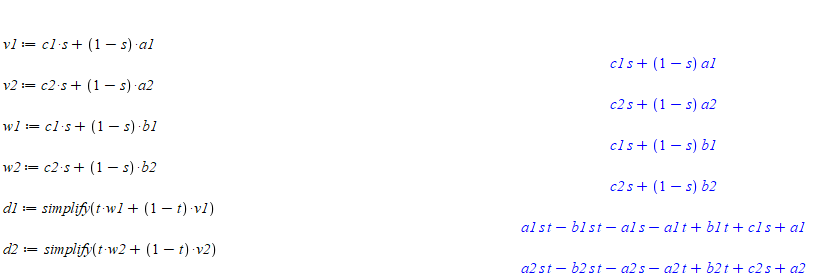
\includegraphics[width=1\textwidth]{tria_mw1.png}
				\centerline{Variablendeklaration}
				\label{fig:Bild1}
			
			
		
		
		
			
				
			\centering
			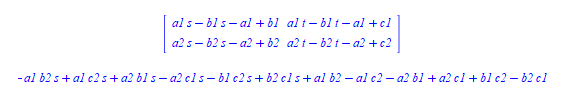
\includegraphics[width=1\textwidth]{mw12.png}
			\centerline{Jacobi-Matrix und Determinantenberechnung}
			\label{fig:Bild1}
			
			
		
			
			
				\centering
				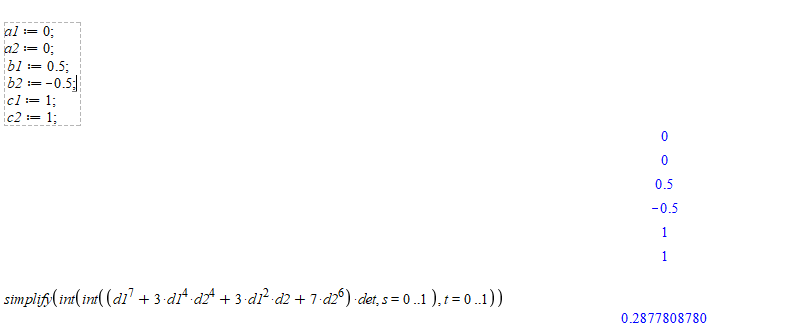
\includegraphics[width=1\textwidth]{tria_mw4.png}
				\centerline{Endresultat}
				\label{fig:Bild1}
						
			
			
	\vspace{4cm}
			
			
			
			\color{change2}
			Implementierung des Codes: \\ 
			
			\color{change}				\lstinputlisting{aufg3_5_1.m} 
			\begin{lstlisting} 
			
			
			\end{lstlisting} 
			\color{change2}Plot:
				
				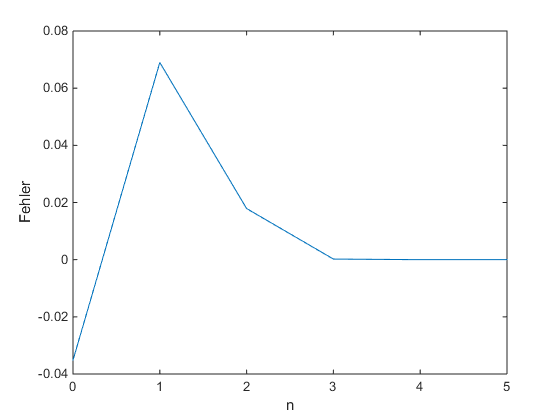
\includegraphics[width=0.7\textwidth]{plot1.png} %70% der Textbreite
				\\
				\centerline{Plot 3.5.1}
			
				
				\color{change2}
			
				


\vspace{2.5cm}				
			\flushleft $-f(x,y)=\sin(50x)\sin(50y), G=conv\{(1,0),(10.2),(3,4)(-1,1)\})$
				
			
				
							
	\color{change}
	\lstset{ 
		language=Matlab, 
		showstringspaces=false}
	
	\lstinputlisting{aufg3_5_2.m} 
	\begin{lstlisting} 
	\end{lstlisting}
				
				
				
				
						\color{change2}
							\centering
							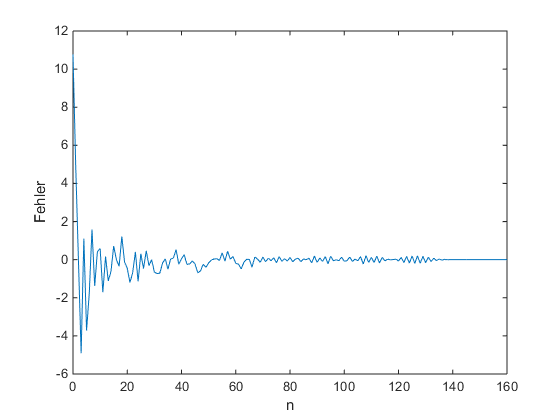
\includegraphics[width=0.7\textwidth]{plot2.png} \\
							\centerline{Plot 3.5.2}
					\hspace{0cm}		
							\label{fig:Bild1}
						
				
			
				\vspace{2cm}
				
\color{change2}
		\flushleft	 $-f(x,y)= \sqrt{\frac{9y}{(1-x^2)}} , G=\hat{Q} $
			
					
					\color{change}
				\lstset{ 
					language=Matlab, 
					showstringspaces=false}
				
				\lstinputlisting{aufg3_5_3.m} 
				\begin{lstlisting} 
				
				
				\end{lstlisting}
				\color{change2}			
				
				
				\color{change2}
				\begin{centering}
					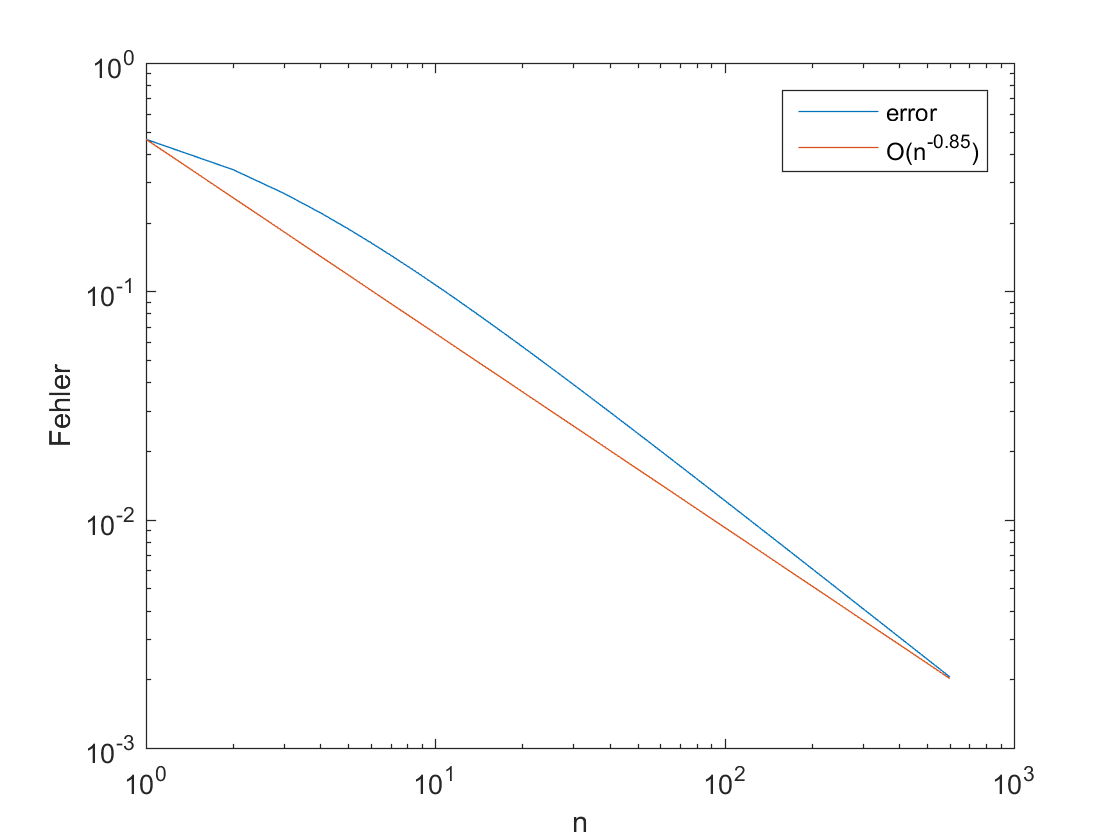
\includegraphics[width=0.7\textwidth]{plot_3_5_3.png} \\
					\centerline{Plot 3.5.3}
					\hspace{0cm}		
					\label{fig:Bild1}
				\end{centering} \\
			
			
					$ -f(x,y) = \begin{cases} 
					1, x^2+y^2 \leq 1 \\
					0, sonst
					\end{cases} , G=\mathbb{R}^2$
					
						\textit{Hinweis:} Approximieren Sie den Kreis durch ein n-Eck.
						Verwenden Sie die letzten beiden Beispiele um $\pi$ zu approximieren.
						Nehmen Sie als Referenzwert bei allen Integralen den analytisch bestimmten Integralwert, sofern dies mölgich ist und stellen Sie die Fehler grafisch dar.\\ Betrachten wir folgende Skizze:\\
						
						\vspace{14mm}
						\hspace{2.7cm}
						\begin{tikzpicture}
							\draw[line width=0mm,red] (0,0)--(2.3,0) node [below] {$b$};
							\draw[line width=0mm,blue] (1.2,1.2) -- (1.2,1.2) node [right=0.5cm] {$\tilde c_2$};
					\draw[thick,->,blue] (-3,0)--(3,0) node[below] {$x$}; % x axis
					\draw[thick,->,blue] (0,-3)--(0,3) node[left] {$y$}; % y axis
				
					\draw[red,thick] (0,0) circle (2.5cm) node[below left] {$a$};
					\draw[blue](0,0) -- (1.75,1.75) node [above right] {$\tilde{c}$};
					\draw[blue](1.75,0) -- (1.75,1.75) node [below=1.75cm] {$\tilde c_1$};
					\draw[red] (2.5,0) -- (0,2.5) node [above right] {$c$};
					\draw[blue](1.25,1.25) -- (1.25,0)   node [below left] {$x_1$};
					\draw [blue] (1.25,1.25) -- (1.25,0.75) node[below right=-0.05cm] {$x_2$};
					
					
						\end{tikzpicture}\\
					\vspace{1cm}
					Durch den Satz von Pythagoras ergibt sich: \\ 
					\vspace{0.5cm} 
					\centerline{$x=(\frac{a_1+b_1}{2},\frac{a_2+b_2}{2}))$.}  
					\vspace{0.5cm}
					Weiters folgt 
					\vspace{0.5cm}
					 
					\centerline{$tan \gamma = \frac{x_2}{x_1} = \frac{\sin\gamma}{\cos\gamma} = \frac{\tilde(c_2)}{\tilde(c_1)}$.} 
					\vspace{0.1cm}
					Wir wissen aus\\
					\vspace{7mm}
					
					
					
				\centerline{$	\sin(x)^2+\cos(x)^2=1$} 
						, dass \\
						\vspace{5mm}
	 
\centerline{$\tilde c_1^2+\tilde c_2^2=1 \Rightarrow \tilde c_1^2+\tilde c_1^2*\frac{(x_2)^2}{(x_1)^2}= 1. $}
\vspace{5mm}
	
			
					
					Daraus ergibt sich wiederum
					\vspace{5mm}
				
		\centerline{	$\tilde c_1\frac{x_2}{x_1}=\tilde c_2$ und $\tilde c_1^2(1+\frac{(x_2)^2}{(x_1)^2})=1$}.
			
				
			\vspace{-2mm}		
					Somit erhalten wir  \\
					\vspace{7mm}
					
					\centerline
					{$\tilde c_2=\frac{x_2}{x_1}* \sqrt{\frac{1}{(1+\frac{(x_2)^2}{(x_1)^2})}}$ und
				$\tilde c_1 = \sqrt{\frac{1}{(1+\frac{(x_2)^2}{(x_1)^2})}}$}
					
				\vspace{3mm}
					
					und schließlich als Endresultat \\
			\vspace{5mm}
					\hspace{4cm}$\frac{x_2}{x_1}=$$\frac{\frac{c_2+b_2}{2}}{\frac{c_1+b_1}{2}}$$=\frac{c_2}{c_1+1}$
						
						
						%$\frac{\frac{c_2+b_2}{2}}{\frac{c_1+b_1}{2}}$
						
					
						\color{change2}.
					
					\vspace{2mm}
						
					Dieses Verfahren wird nun iterativ angewandt um das gewünschte Resultat zu erreichen.
					\vspace{3mm}
					Der folgende Code repräsentiert dies:
					
					
						
					\color{change}
				\lstset{ 
					language=Matlab, 
					showstringspaces=false}
				
				\lstinputlisting{aufg3_5_4.m} 
				
				
				\color{change2}
				Der folgende Plot veranschaulicht das Resultat graphisch: (loglog Plot missing)
				\vspace{-2mm}	
						\centering
						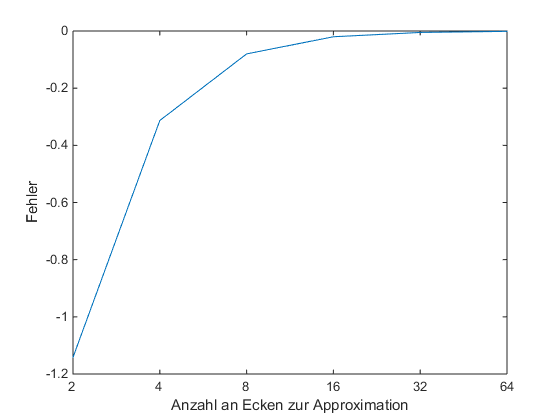
\includegraphics[width=0.7\textwidth]{plot4.png} \\
						\vspace{2mm}
						\centerline{Plot 3.5.4}
						\label{fig:Bild1}
					
					
				
				
		
		
	
			
	
	
		
	
			 
		
	
	


\end{document}